%Nama Kelompok : Five Group BSD
%Anggota :
%Dwi Yulianingsih
%Arjun Yuda Firwanda
%Jeremia Wahyudi Sianturi
%Dwi Septiani Tsaniyah
%Ervanda Rambu Anarky

\section{hardware}
Dalam sebuah sistem komputer terdapat perangkat keras(Hardware), perangkat keras (Hardware) didefinisikan sebagai komponen-komponen komputer yang dapat ditangkap dengan indra peraba kita. Hardware dalam sistem komputer dibagi menjadi dalam beberapa bagian diantaranya adalah
1. Perangkat Input 
2. Perangkat Proses 
3. Perangkat output. 
Perangkat Input atau output sering dikenal dengan istilah I/O device atau Input / Output Device. I/O device ini adalah perangkat-perangkat komputer yang digunakan untuk masukan dan keluaran. I/O device ini bisa terdapat di dalam atau di luar CPU. Perangkat yang terdapat di luar CPU dikenal dengan istilah Periferal l. Jadi saya yakin contohnya sudah bisa kalian tebak dan sebutkan tentunya.
\ref{hardware.png}
Contoh gambar 

\begin{figure}[ht]
\centerline{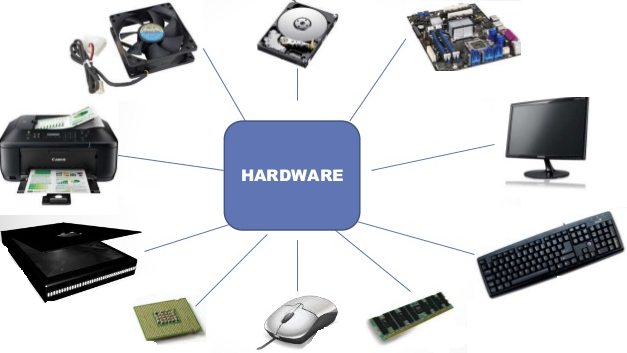
\includegraphics[width=1\textwidth]{figures/hardware.png}}
\caption{gambar hardware}
\label{hardware.png}
\end{figure}

\subsection{Cara Kerja Hardware}
Perangkat yang berada di luar CPU diantaranya adalah Keyboard, mouse, monitor ataupun printer. Sedangkan perangkat yang terdapat dalam CPU dikenal dengan istilah Storage Device. Contoh storage device ini seperti Hardisk, CD Room, Disk Drive dan lain sebagainya. Di dalam CPU terdapat CU atau Control Unit, RAM dan ROM. Control unit ada juga yang namanya ALU atau Aritmatic Logical Unit yang berfungsi untuk melakukan berbagai kegiatan yang terkait dengan perhitungan-perhitungan yang dilakukan.
Keyboard Mouse Monitor Printer CPU (Central Processing Unit)/ Perangkat Proses PERANGKAT INPUT/OUTPUT Keyboard ini adalah merupakan alat yang banyak digunakan dan menjadi mutlak untuk di gunakan. Keyboard memiliki fungsi yang mirip dengan mesin ketik pada zaman dahulu. Akan tetapi keyboard ini memiliki  suatu kemampuan lebih yang tidak dimiliki oleh mesin tik pada zaman dulu diantaranya dapat ditemui tombol-tombol fungsi mulai dari F1 sampai dengan F12 yang umumnya digunakan untuk memberikan suatu perintah yang diberikan namun perintah tersebut tergantung daripada aplikasi atau program yang akan digunakan. Keyboard yang selama ini kita gunakan biasanya terdiri atas 2 jenis yakni Keyboard QWERTY dan jenis keyboard DVORAK. Namun keyboard yang sering digunakan dan banyak digunakan saat ini adalah keyboard jenis QWERTY karena lebih mudah digunakan dibandingkan dengan keyboard DVORAK. Dengan pertumbuhan teknologi yang amat pesat membuat keyboard pada masa ini berkembang sangat maju contohnya pada saat ini ada keyboard yang menggunakan wireless system atau tanpa kabel . Struktur-struktur tombol pada keyboard Dari sisi tombol yang digunakan, keyboard memiliki perkembangan yang tidak     terlalu pesat sejak ditemukan pertama kali. Yang terjadi hanyalah penambahan�penambahan beberapa tombol bantu yang lebih mempercepat pembukaan aplikasi program. Secara umum, struktur tombol pada keyboard terbagi atas 4 (empat) , yaitu: � Tombol Ketik (typing keys) Tombol ketik adalah salah satu bagian dari keyboard yang berisi huruf dan angka serta tanda baca. Secara umum, ada 2 jenis susunan huruf pada keyboard, yaitu tipe QWERTY dan DVORAK. Namun, yang terbanyak digunakan sampai saat ini adalah susunan QWERTY. � Numerickeypad adalah bagian khusus dari keyboard yang berisi angka dan berfungsi untuk memasukkan file berupa angka-angka dan operasi perhitungan.Struktur-struktur angkanya disusun menyerupai kalkulator dan alat hitung lainnya. � Tombol Fungsi (Function Keys) Tahun 1986, IBM menambahkan beberapa tombol fungsi pada keyboard standard. Tombol ini dapat dipergunakan sebagai perintah khusus yang disertakan pada sistem operasi maupun aplikasi. � Tombol kontrol (Control keys) Tombol ini menyediakan kontrol terhadap kursor dan layar. Tombol-tombol yang termasuk dalam kategori ini adalah 4 tombol bersimbol panah di antara tombol ketik dan numeric keypad, home, end, insert, delete, page up, page down, control (ctrl), alternate (alt) dan escape (esc). MOUSE Mouse ini adalah sebuah alat yang digunakan sebagai pengatur posisi kursor (tanda panah yang sering kali bergerak ketika kita menggeserkan mouse). Pada awalnya mouse yang ada adalah masih memakai roda di bawahnya, namun dengan perkembangan yang pesat dari tehnologi saat ini mengakibatkan perkembangan perangkat komputer mengalami kemajuan yang luar biasa, saat ini mouse sudah menggunakan tehnologi infrared dan tehnologi wireless. SCANNER Scanner adalah alat yang digunakan secara otomatis untuk memasukkan data baik berupa huruf,Dengan perkembangan teknologi yang semakin pesat, scanner sekrang ini dapat digunakan untuk memasukkan objek dari sebuah benda secara langsung sehingga objek tersebut dapat berupa gambar seperti 3 dimensi. Monitor ini merupakan salah satu perangkat untuk menampilkan informasi yang dihasilkan dari proses input (masukan). Ada 2 jenis Monitor diantaranya Monitor CRT (Cathode Ray Tube) dan Monitor LCD (Liquid Crystal Display). 
Secara garis besar printer memiliki jenis-jenis yang terdiri atas beberapa macam, yaitu :
1. Dot Matrikx Printers, yang bekerja dengan menggunakan cara hentakan. Pada jenis ini sebenarnya printer menghentakkan tinta diatas karbon untuk membuat sebuah karakter yang akan dicetak di kertas. Jenis seperti ini banyak digunakan untuk mencetak slip gaji.
2. Inkjet printers, jenis ini hanya dapat digunakan untuk mencetak dalam jumlah yang sedikit dan tidak mengutamakan kecepatan, contohnya mencetak surat di perkantoran dan mencetak di rumah secara personal.
3. Laser Printers, merupakan jenis alat cetak yang dapat menghasilkan yang sangat baik dan juga menggunakan kecepatan tinggi.
Kemudian ada Speaker, alat ini berfungsi untuk menghasilkan suara yang telah di proses dalam computer. Yang dimaksud perangkat proses adalah perangkat yang dipakai untuk melakukan sekumpulan perintah yang ditujukan untuk menghasilkan suatu hal yang diinginkan. Komponen CPU dibagi menjadi beberapa bagian yang terdiri dari :
4.	Motherboard, merupakan sebuah papan induk yang menyediakan koneksi logic dan elektrik antar komponen-komponen dalam komputer. Pada komputer yang telah modern alat ini merupakan sebuah PCB yang kompleks dan berisi komponen dan interkonektor semacam slot dan soket. Dalam motherboard minimal terdiri dari : - Soket Microposesor �Slot ke memori utama dan �Chipset yang menjadi perantara antar CPU dan Font-side bus yang memiliki fungsi untuk mengendalikan perangkat input/outpus lainnya. 
5. Memori merupakan perangkat keras yang digunakan untuk menyimpan data. Berdasarkan sifat data yang disimpan maka memori di kelompokkan dalam : 
a. ROM 
Read Only Memory adalah media penyimpanan data pada komputer. ROM bersifat permanen artinya program atau data yang disimpan di dalam ROM tidak mudah hilang atau berubah walaupun aliran listrik dimatikan.  ROM di dalam komputer modern berupa IC. File-file  yang ada dalam ROM dimasukkan langsung melalui mask pada waktu perakitan chip, dan tentunya hal ini yang membuatnya sangat ekonomis terkhususnya jika kita memproduksi dalam jumlah yang banyak. Namun hal ini juga yang membuatnya mahal karena bersifat tidak fleksibel. Sebuah perubahan walaupun hanya 1 bit membutuhkan mask baru yang barang tentunya tidak murah. RAM (Random Akses Memory) merupakan sebuah jenis dari penyimpanan komputer yang isinya dapat diakses dalam waktu yang tidak menentu tidak memperdulikan letak data tersebut dalam memori. Perusahaan semikonduktor yang mulai debut pertamanya memproduksi RAM ini adalah INTEL dengan memproduksi RAM dengan tipe DRAM. Saat ini dipasaran juga bisa dijumpai jenis-jenis/ tipe RAM diantaranya jenis dari DDR 3. Processor Adalah lempengan khusus berisi rangkaian IC (Integrated Circuit) yaitu kumpulan transistor terpadu dalam satu silikon, contohnya Intel, AMD. Processor dipakai untuk memproses sebuah data atau program yang akan dimasukkan melalui peralatan input. 4. BIOS Adalah merupakan singkatan dari Basic Input Output System. BIOS merupakan semacam software yang langsung terinstal dalam chip yang dijalankan oleh PC manakala komputer dihidupkan. Fungsi BIOS adalah mengidentifikasi serta menganalisis komponen-komponen perangkat keras seperti hardisk, CD, Floopy untuk mencari program lain pada perangkat keras tersebut yang dapat mengendalikan PC (Sistem Operasi). Proses ini dikenal dengan istilah booting atau booting up. 5. Sound Card Adalah suatu perangkat keras komputer yang digunakan untuk mengeluarkan suara dan juga untu merekam suara. Pada mulanya soundcard ini hanya dapat sebagai pelengkap pada sebuah PC akan tetapi saat ini soundcard bisa dikatakan merupakan perangkat yang harus ada pada PC. Ada beberapa tipe soundcard : 
a. Soundcard yang on board artinya soundcard yang menempel langsung pada sebuah motherboard 
b. Sound card offboard artinya sound card yang pemasangannya dilakukan pada slot ISA/ PCI yang ada pada motherboard c. Sound card external yakni sound card yang penggunaannya disambungkan ke PC dengan jalan menghubungkan melalui port eksternal seperti USB. 
6. VGA (Video Grafhics Adapter) Adalah merupakan perangkat keras pada PC yang dapat mendisplay gambar melalui konektor. Perangkat ini terhubung ke motherboard melalui PCI, AGP, serta PCI express.
7. Hardisk Adalah merupakan perangkat keras komputer yang digunakan sebagai media penyimpan data (storage) dan termasuk salah satu memory eksternal dalam komputer. Saat ini bentuk fisik dari Hardisk menjadi semakin tipis dan kecil namun mempunyai kapasitas penyimpanan yang sangat besar. Bukan hanya Hardisk sebagai perangkat internal dari sebuah PC (komputer) tetapi juga dapat dipasang diluar perangkat dengan penggunaan kabel USB.
8. PCI (Periferal Component Interconnect) merupakan bus khusus pada komputer yang berfungsi sebagai tempat menancapkan perangkat-perangkat periferal ke motherboard. PCI express pada sistem unit komputer merupakan penyederhanaan dari PCI sebagai slot untuk kartu tambahan. PCI express di desaign dengan tujuan sebagai pengganti fungsi dari bus PCI. Motherboat Hardisk Memori Processor Hardware dalam sebuah sistem komputer, perangkat keras (Hardware) diartikan sebagai komponen-komponen komputer yang dapat ditangkap dengan indra peraba kita. Hardware dalam sistem operasi komputer dibagi menjadi dalam beberapa bagian diantaranya yaitu : 
1.	Perangkat input
2.	Perangkat proses
3.	Perangkat output.
Perangkat masukan (input) atau keluaran (output) kita kenal dengan sebutan I/O device atay Input/output device. I/O device ini merupakan perangkat-perangkat computer yang kita gunakan untuk masukan dan keluaran. I/O device ini terdapat didalam maupun diluar CPU. Perangkat yang ada diluar dari CPU biasa kita kenal dengan periferal. Perangkat yang ada di luar CPU diantaranya adalah Keyboard, Mouse, Monitor, maupun Printer. Perangkat yang berada diluar CPU biasa kita kenal dengan istilah Storage Device yang berisi Hardisk, CD room, Disk Drive dan lainnya.  
Di dalam CPU (Central Proseseing Unit) terdapat CU ( Control Unit), RAM (Random Akses Memory) dan ROM (Read Only Memory). CPU adalah sebuah perangkat keras komputer yang dapat memahami dan dapat melaksanakan perintah. CPU terletak motherboard. CPU juga sering disebut otak Komputer karena CPU semua aktivitas dan jalannya proses semua program, termasuk aplikasi ataupun software.  Berikut komponen didalam CPU:
1.	Unit Kontrol
Yang mengatur segala proses jalannya program, sehingga menjadi singkron antara komponen dan program.
2.	Register
Adalah sebuah perangkat penyimpan kecil yang memiliki akses atau jaringan yang cukup tinggi yang dapat menyimpat data atau file dan intruksi yang sedang dijalankan.
3.	Unit ALU (Aritmatic Logical Unit)
Yang melakukan operasi aritmatika dan operasi logika yang berkenaan dengan proses perhitungan. ALU memiliki bagian yang pertama aritmatika satuan dan boolean unit logika yang masing-masing mempunyai ciri dan perintah yang berbeda. Tugas utama ALU ialah mengenai perhitungan aritmatika.
Jenis-jenis CPU Komputer
1.	Intel Processor
2.	AMD (Advanced Micro Processor)
3.	ARM Processor
4.	Cyric Processor
5.	Transmeta Processor
6.	Via
7.	Apple Processor
8.	IBM Processor
9.	IDT Processor
Fungsi CPU:
1.	Fetching, Adalah proses pengambilan atau pemanggilan data.
2.	Decoding, Adalah penerjemahan program ke dalam bahasa yang dimengerti oleh CPU.
3.	Excuting, Adalah melakukan kalkulasi data perhitungan dengan ALU.
4.	Storing, Adalah penyimpanan data.
Jadi Control ini berfungsi untuk mengatur dan menjalankan instruksi dalam urutan yang telah ditetapkan. Selain CU (Control Unit) dan ada juga yang namanya ALU (Aritmatic Logical Unit) yang berfungsi melakukan berbagai kegiatan ataupun tugas yang terkait dengan perhitungan-perhitungan.  Kita dapat membuat perintah apapun yang mengenai tugas ataupun project yang akan kita buat.

dalam artikel ini kami mengutip beberapa hal dari \cite{komputer2006sgs} dan dari \cite{tanenbaum2009modern}
Semua hal yang diciptakan oleh  manusia pasti memiliki kelebihan dan kekurangan, sama hal nya dengan hardware. Mari kita jabarkan kelebihan dan kekurangan dari perangkat keras ini :
Kelebihan dari hardware ini adalah perangkat keras ini bias dimodivikasi menjadi berbagai bentuk sesuai kebutuhan penggunanya
Kekurangan dari perangkat keras ini adalah ukurannya yang cukup memakan tempat membuat kita agak sulit untuk mengaturnya.

Contoh gambar 
\ref{diskdrive.jpg}
\begin{figure}[ht]
\centerline{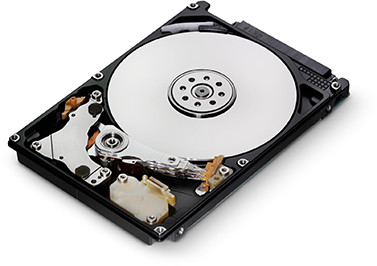
\includegraphics[width=1\textwidth]{figures/diskdrive.jpg}}
\caption{gambar diskdrive}
\label{diskdrive.jpg}
\end{figure}

Contoh gambar \ref{monitor.jpg} 

\begin{figure}[ht]
\centerline{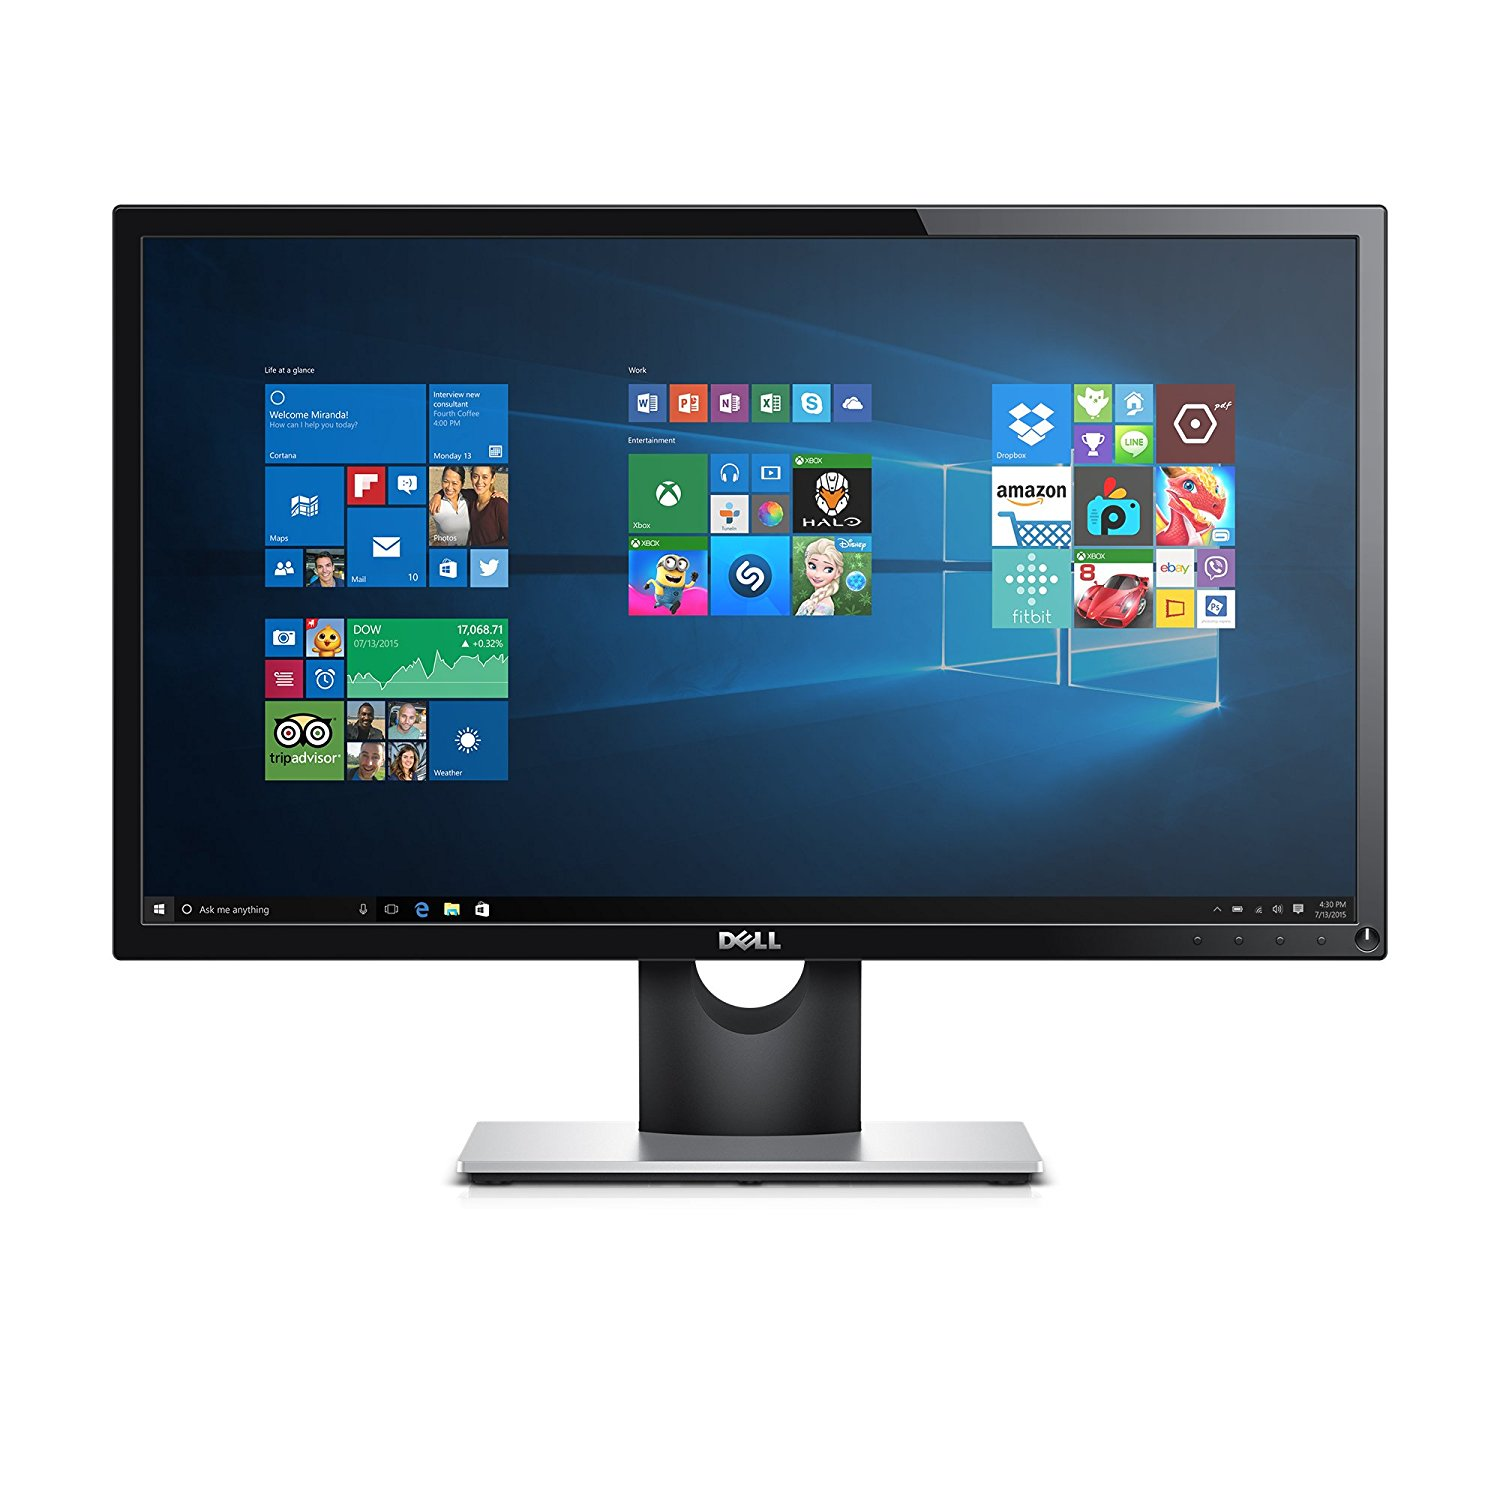
\includegraphics[width=1\textwidth]{figures/monitor.jpg}}
\caption{gambar monitor}
\label{monitor.jpg}
\end{figure}

Contoh gambar \ref{m100-gallery.png}

\begin{figure}[ht]
\centerline{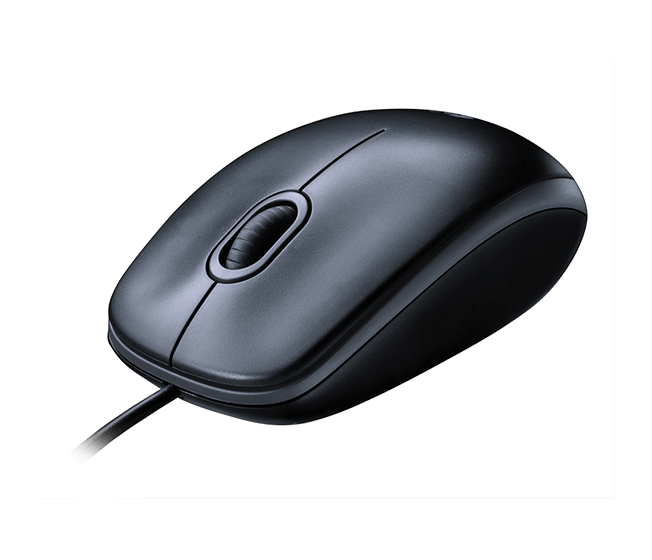
\includegraphics[width=1\textwidth]{figures/m100-gallery.png}}
\caption{gambar mouse}
\label{m100-gallery.png}
\end{figure}

Contoh gambar \ref{41skLxWQtyL.jpg}

\begin{figure}[ht]
\centerline{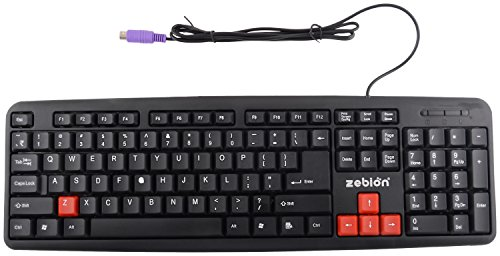
\includegraphics[width=1\textwidth]{figures/41skLxWQtyL.jpg}}
\caption{gambar keyboard}
\label{41skLxWQtyL.jpg}
\end{figure}

\section {kesimpulan}
Cara kerja hardware atau perangkat keras itu bermacam-macam. Dalam hardware kita dapat menemukan banyak perangkat yang diantaranya ada keyboards, mouse, monitor, cpu, dan lain sebagainya. Kita sangat sering menggunakan perangkat2 ini akan tetapi kurang memahami bagaimana cara perangkat ini bekerja. Oleh karena itu dengan adanya teknologi yang telah berkembang pesat kita bias mengakses hal-hal sepele yang ingin kita ketahui seperti contohnya hardware ini. Hardware atau perangkat keras sangat membantu kita dalam memudahkan menggunakan computer dapat kita bayangkan apabila tidak ada hardware pastinya computer tidak akan berjalan sesuai dengan apa yang kita inginkan. Kita tidak dapat menulis, mengontrol maupun memerintahkan computer kita untuk melakukan hal-hal yang ingin kita lakukan maupun kita butuhkan, dengan adanya hardware atau perangkat keras ini kita dapat dengan mudah menggunakan computer dan mengakses hal-hal yang akan kita gunakan maupun kita inginkan. Dengan adanya cara kerja hardware kita dapat menjalankan computer kita. Karena computer pada zaman ini merupakan hal sangat penting dan importan dalam kemajuan saat ini maka kita juga harus dengan hati-hati mengikuti perkembangan jaman pada era ini. Hardware didefinisikan sebagai perangkat-perangkat yang ada dan melekat dalam computer yang dapat kita pegang ataupun kita raba, hardware computer dibagi menjadi dua yaitu perangkat masukan dan perangkat keluaran. Perangkat masukan ialah perangkat yang ada di dalam computer itu sendiri, jika perangkat keluaran yaitu perangkat yang ada di luar dari computer tersebut. Jadi itulah kesimpulan yang dapat diambil dari artikel ini semoga bermanfaat dan dapat kita terapkan di kehidupan sehari-hari.
